Normally \ce{N2} would not be a good choice, due to the fact that \ce{N2H+} has the same mass as the formyl isomers at $m/z=29$, but we may instead introduce \ce{^{15}N2} to produce a new peak at $m/z=31$. We do not expect and do not see any reaction between the initially loaded ions of \ce{Be+} and \ce{C+} making this the ideal candidate for titration. But according to \cref{tab: affinities}, we should still have a separation of the isomers, thus:

\begin{align}
	\ce{Be+ + ^15N2 & -> no reaction} \nonumber \\
	\ce{C+ + ^15N2 & -> no reaction} \nonumber \\
	\ce{HCO+ + ^15N2 & -> no reaction} \label{r: HCO+N2->NA} \\
	\ce{HOC+ + ^15N2 & -> ^15N2H+ + CO} \label{r: HOC+N2->N2H}
\end{align}

To verify reaction \ref{r: HOC+CO->HCO}, trapped \ce{Be+} and \ce{C+} ions are exposed to the water from the CBGB at a density of $4.3 \times 10^6$ cm$^{-3}$ while simultaneously flooded with $\approx 3 \times 10^7$ cm$^{-3}$ of \ce{CO} from the leak valve connected to the differential pumping region such that $k_{\ref{r: HOC+CO->HCO}} \gg k_{\ref{r: C+H2O->HCO}, \ref{r: C+H2O->HOC}}$. After 10 s, the gate valve between the differential pumping and experimental ion chamber regions is manually closed, after which, $10^9$ cm$^{-3}$ of \ce{^15N2} is introduced for 10 s. A TOF trace for this procedure is shown in figure \ref{fig: CO N2 TOF}.

\begin{figure}[H]
	\centering
	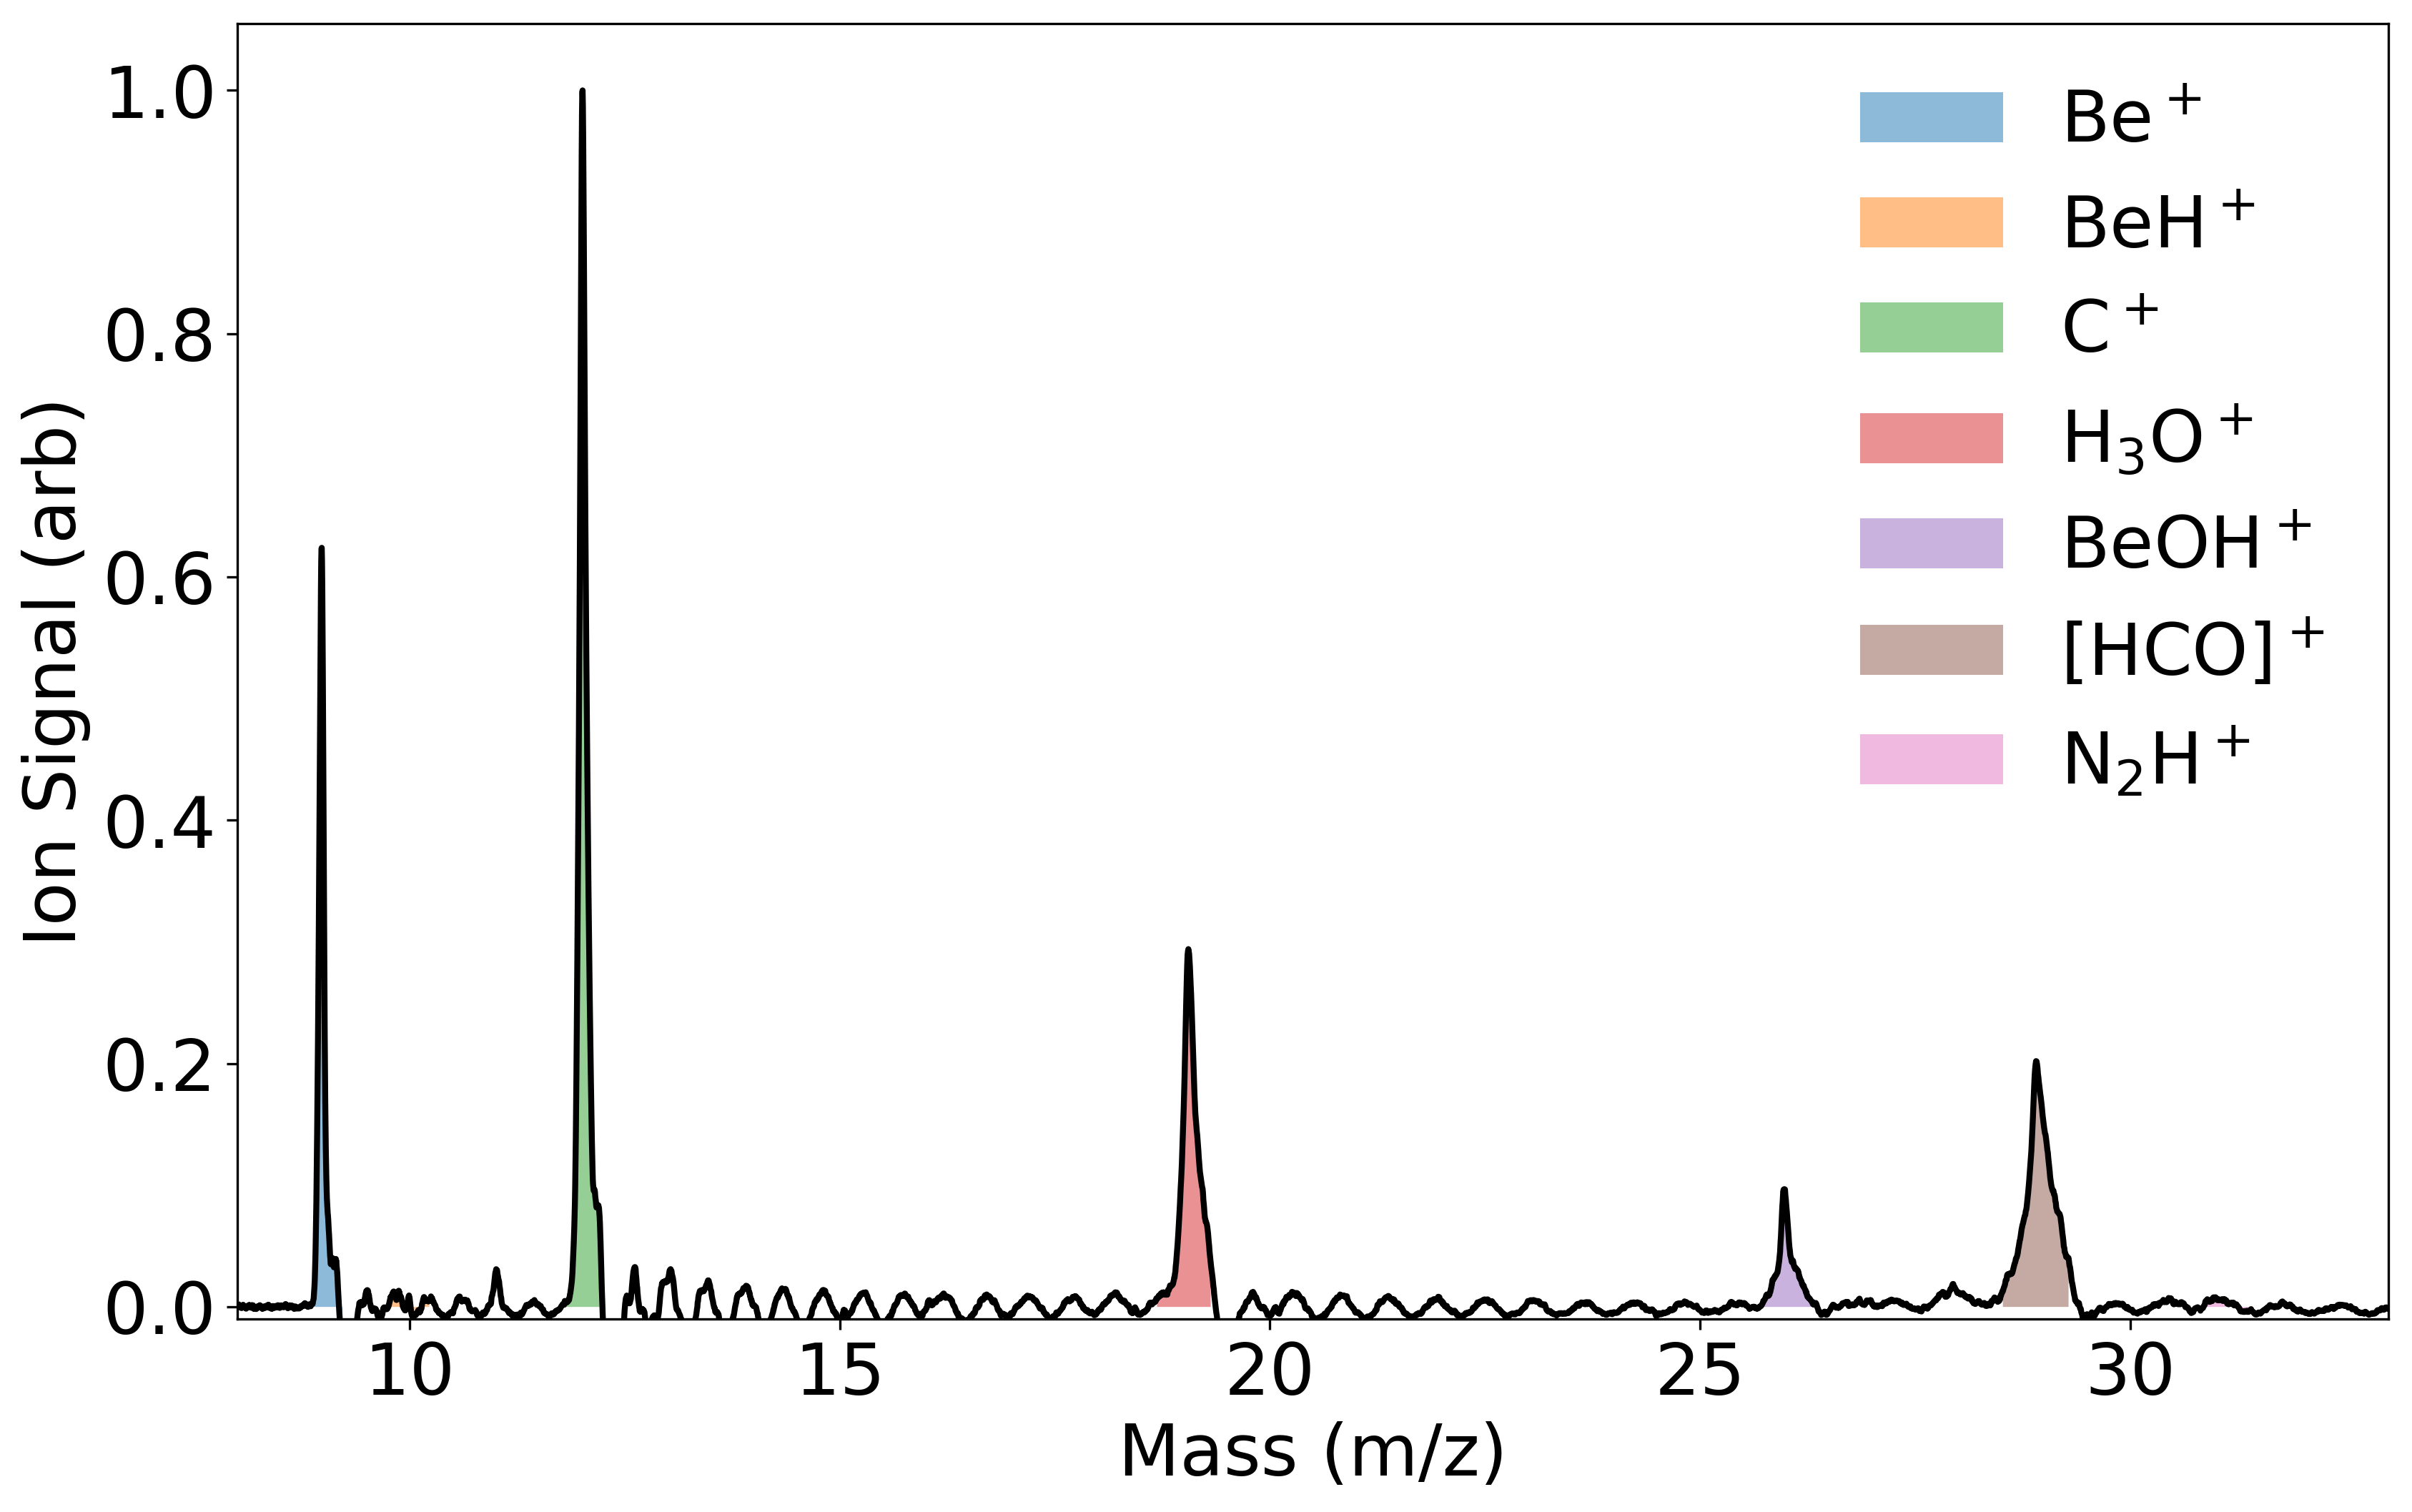
\includegraphics[width=0.8\textwidth]{images/C_H2O_CO_15N2.png}
	\caption{TOF trace of reaction products of \ce{Be+} and \ce{C+} after exposure to both water from the CBGB beam, and \ce{CO} (10 s) before titration with \ce{15N2} (10 s). There is a distinct lack of \ce{N2H+}, indicating full conversion of \ce{HOC+ -> HCO+}.}
	\label{fig: CO N2 TOF}
\end{figure}

Integrated \ce{N2H+} signal was found to be below the threshold for null signal demonstrating both points that reaction \ref{r: HOC+CO->HCO} proceeds as expected, as well as experimental verification that reaction \ref{r: HCO+N2->NA} does not occur.

At room temperatures, the branching ratio has been found to be approximately 84:16 (\ce{COH+}:\ce{HCO+})\cite{Freeman1987}, but unexplored at lower regimes.

To determine the branching ratio, \ce{Be+} and \ce{C+} in the trap are exposed to the CBGB for 10 s, after which, the gate valve connecting the differential pumping region and ion trap chamber is closed. \ce{^15N2} is then introduced via leak valve to react with the \ce{HOC+}. Only runs taken at delay times of 10 s were taken, as we only concern ourselves with a ratio of signals. Repeating this process over various densities of \ce{^15N2} allows us to determine the isomer branching ratio. We expect the ratio of \ce{N2H+} and \ce{[HCO]+} to follow the form:

\begin{equation}
	\frac{\ce{^{15}N2H+}(t)}{\ce{^{15}N2H+}(t)+\ce{[HCO]+}(t)} = C \left( 1-e^{-k_{\ref{r: X+HOC->XH}} \rho t} \right)
	\label{eq: N2 asymptote}
\end{equation}

A fit performed on the data over various densities yields a rate constant of $k_{\ref{r: X+HOC->XH}} = ((6.6 \pm 1.0) \times 10^{-10})$ cm$^3$/s, and a final branching ratio of $\ce{HOC+}:\ce{HCO+} = 0.58 \pm 0.01$, in good agreement with the \ce{CO2} titration results.

\begin{figure}[H]
	\centering
	\makebox[\textwidth][c]{
	\begin{tabular}{cc}
		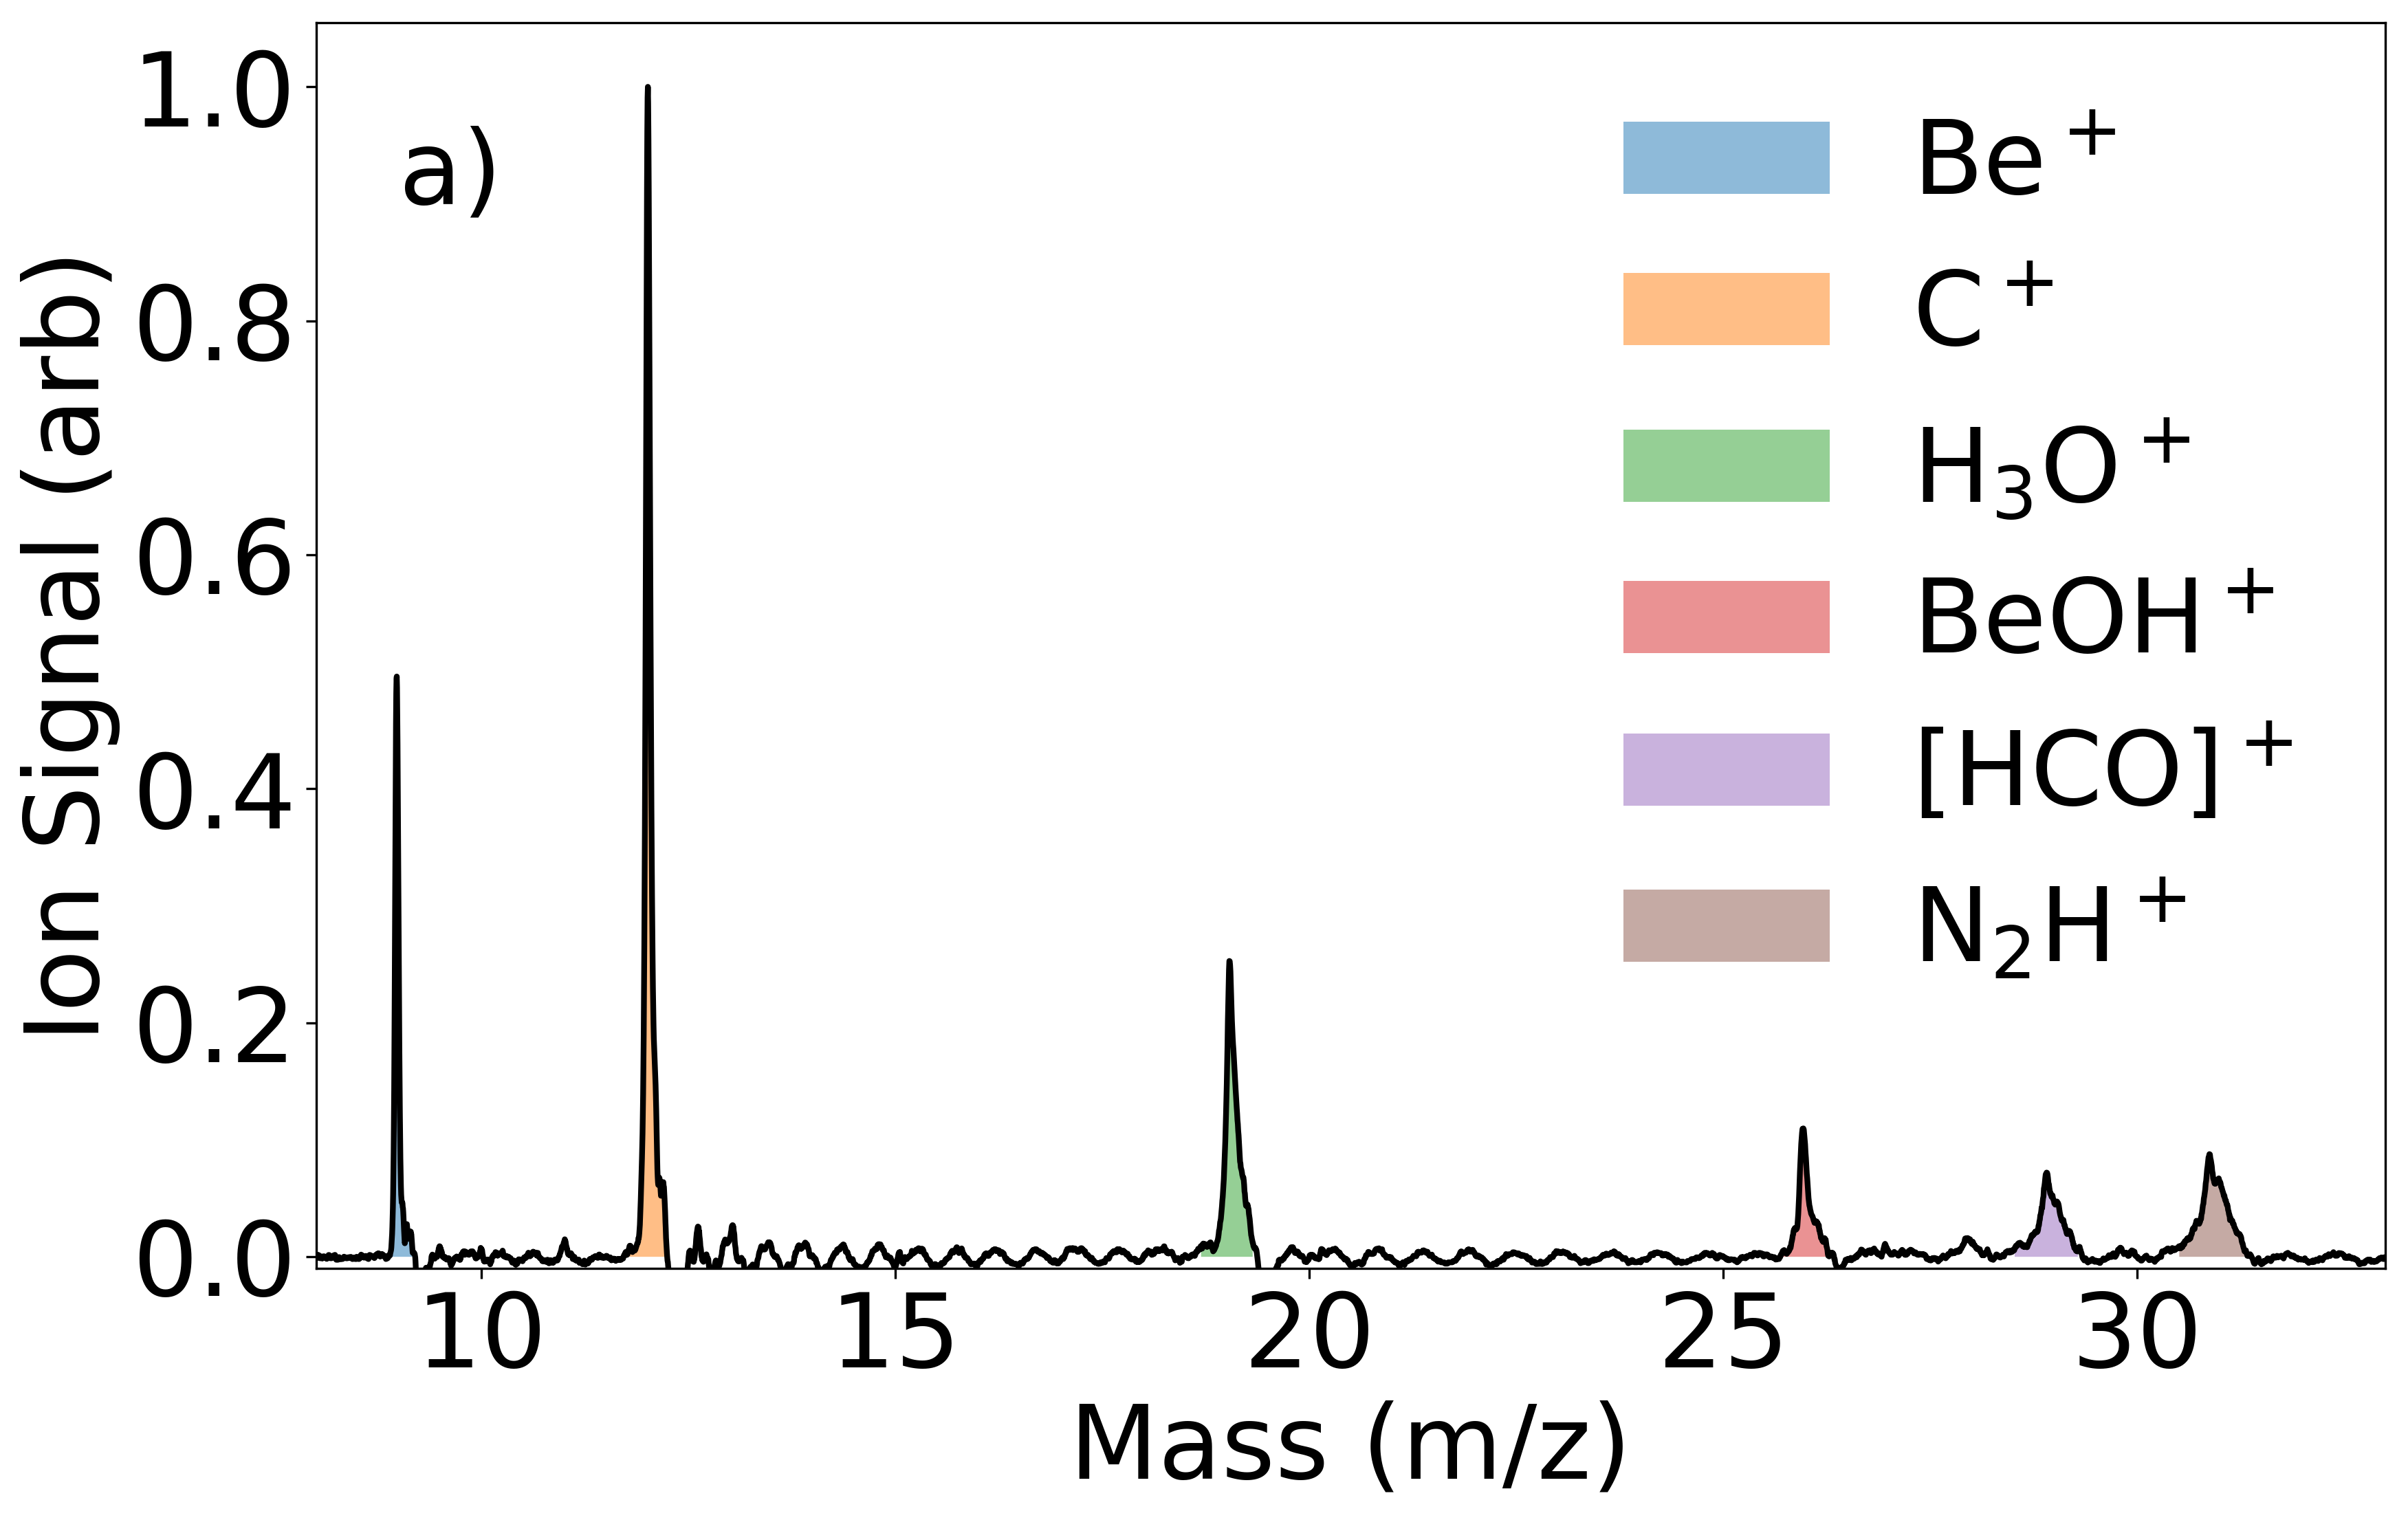
\includegraphics[width=0.5\textwidth]{images/C_H2O_15N2_small.png} &
		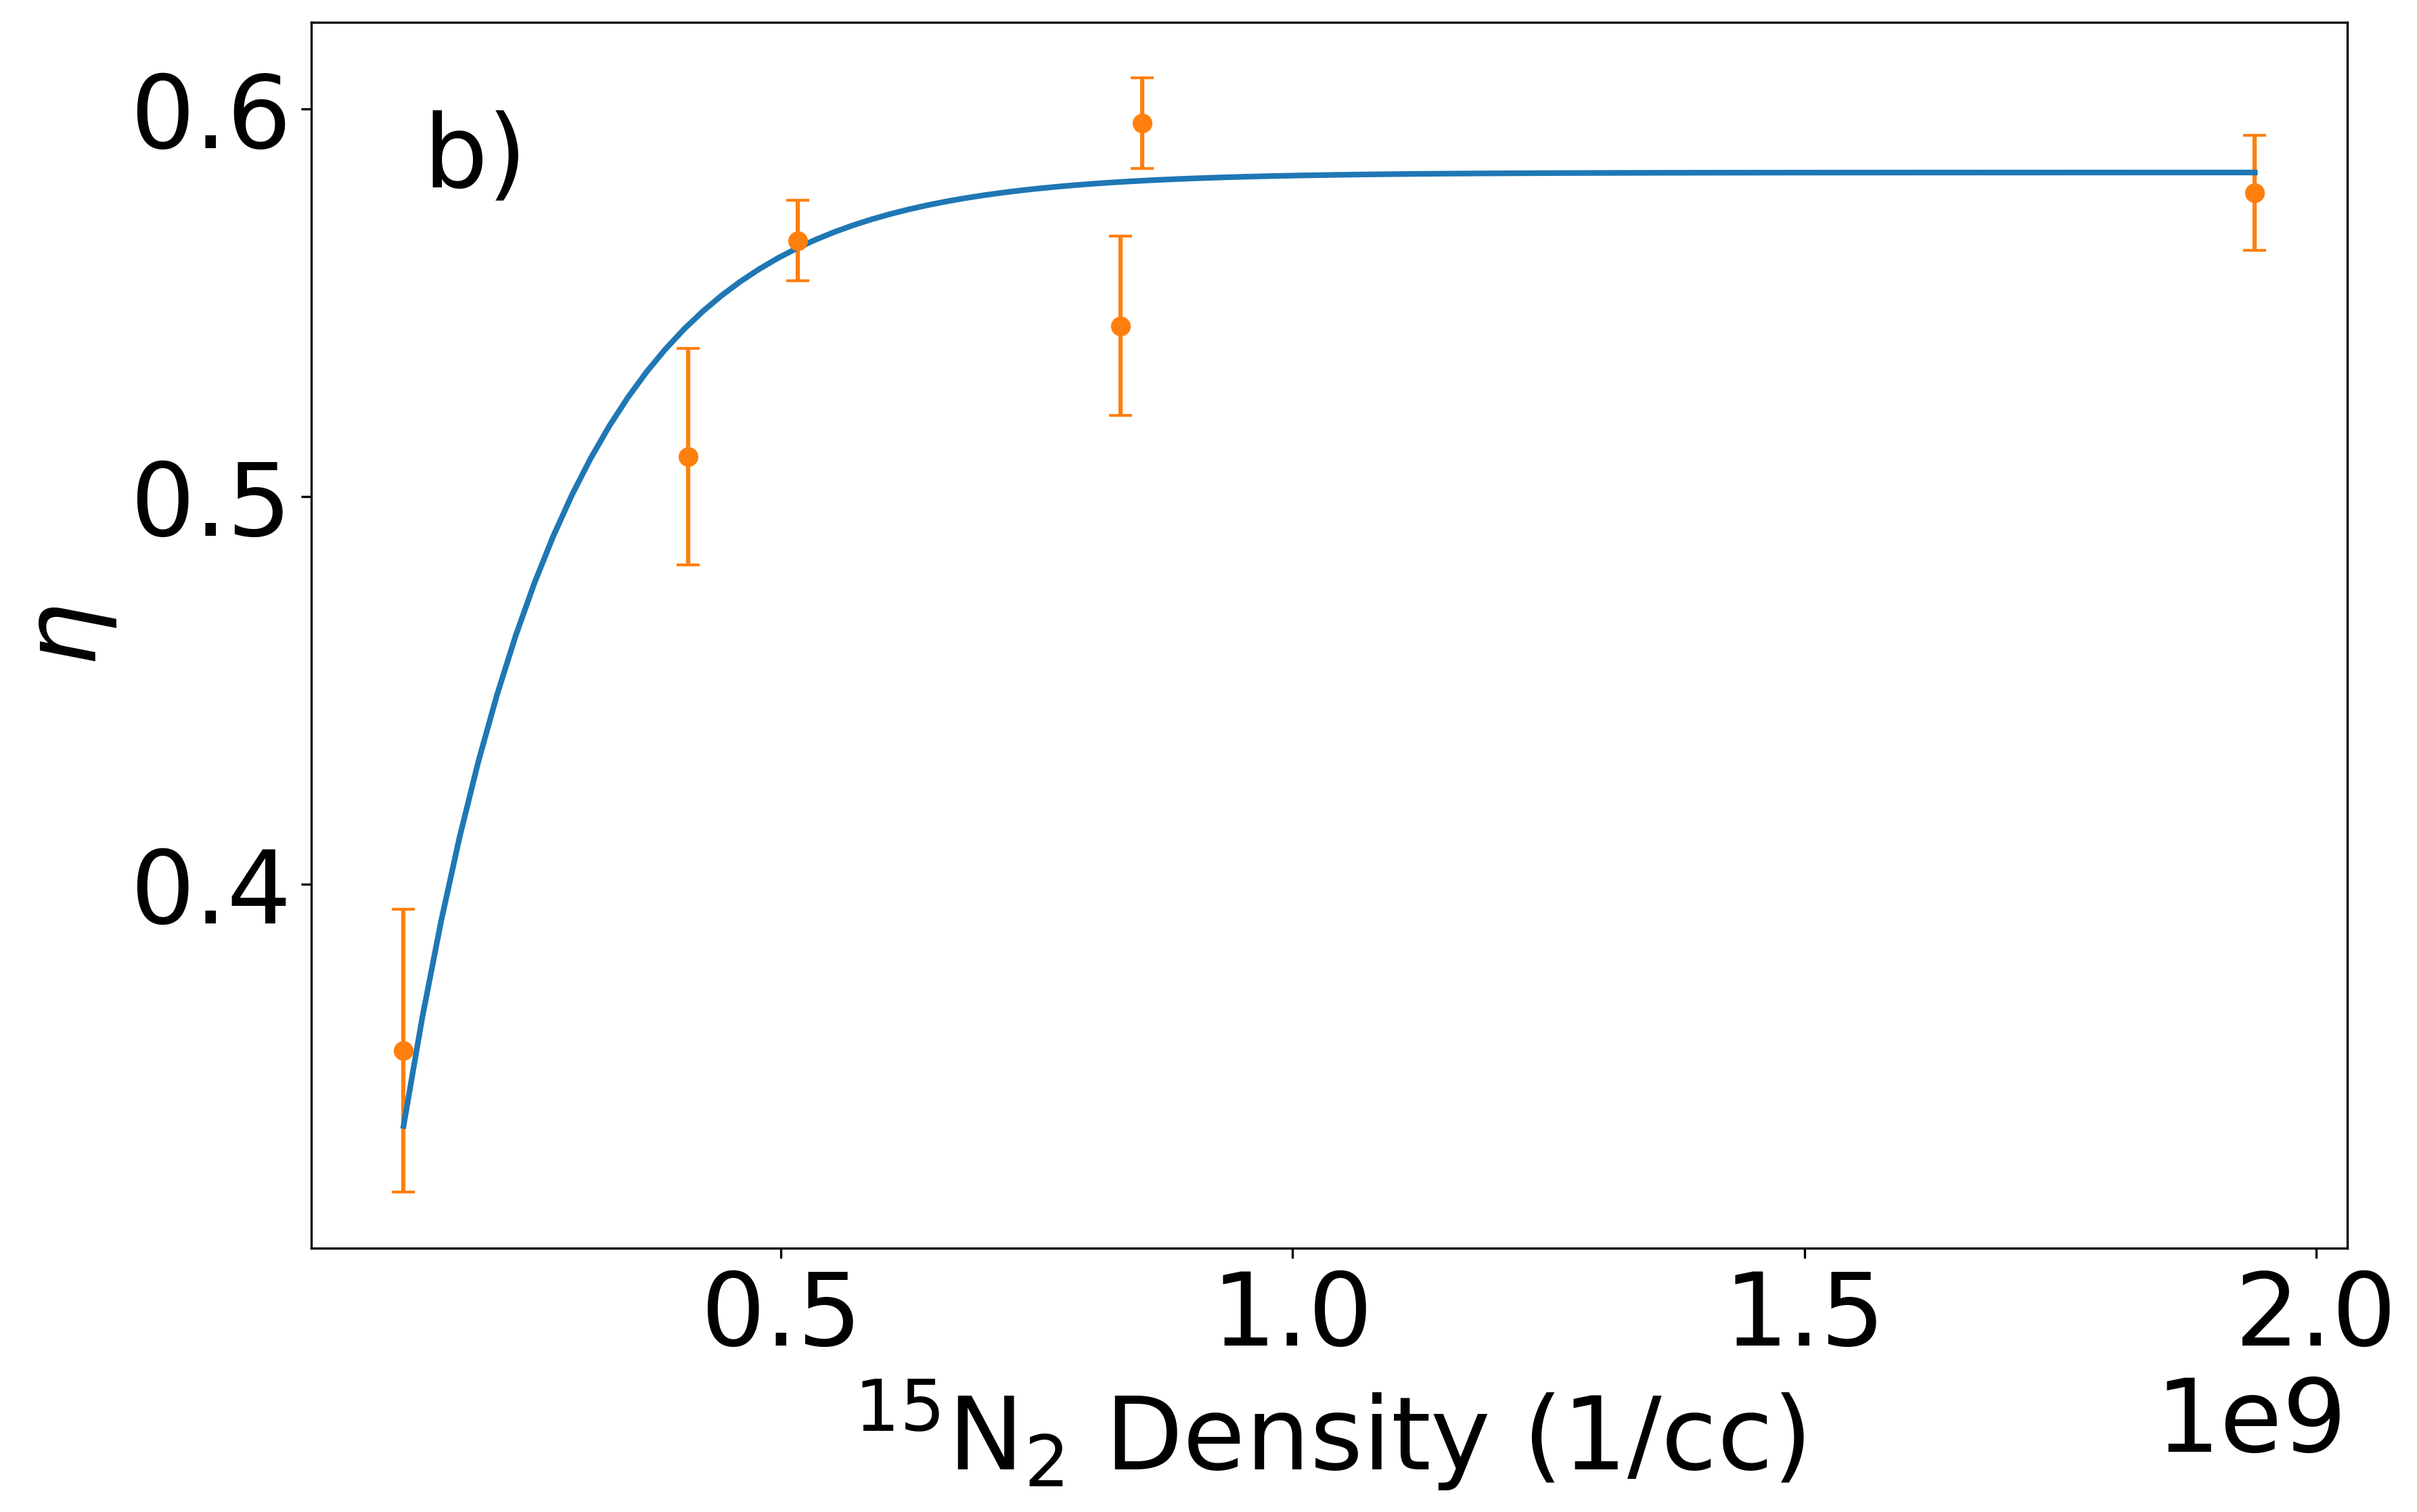
\includegraphics[width=0.5\textwidth]{images/N2_pressure_scan_small.png}
	\end{tabular}
	}
	\caption{a) Average of 10 TOF traces of \ce{Be+} and \ce{C+} exposed to water from the CBGB (10 s), then exposed to \ce{^15N2} from the leak valve (10 s) at a density of $1 \times 10^9$ cc$^{-1}$. b) The fraction of the titrated isomers, $\eta \equiv \ce{^{15}N2H+}/(\ce{^{15}N2H+}+\ce{[HCO]+})$, as a function of \ce{^15N2} density. Fitted parameters yield values $C = 0.58 \pm 0.01$, $k_{\ref{r: X+HOC->XH}} = ((6.6 \pm 1.0) \times 10^{-10})$ cm$^3$/s.}
	\label{fig: N2 pressure scan}
\end{figure}

To estimate a limit on the isomerization, we consider the above reactions \ref{r: X+HOC->HCO} and \ref{r: X+HOC->XH}, where \ce{X = ^{15}N2} in the context that we can only determine the abundance of \ce{[HCO]+} and \ce{^{15}N2H+}. As a function of pressure, we cannot see reaction \ref{r: X+HOC->HCO}, but if it does contribute, we should see a discrepancy in the total rate constant, which we estimate to be Langevin: $k_L = 8.0 \times 10^{-10}$. This gives us a possible isomerization rate of 22\%, which then yield a branching ratio of 70:30.
%CO with beam
%
%k1: 7.39e-02, 5.88e-03
%k2: 2.23e-01, 2.02e-02
%C0: 8.25e-01, 7.11e-02
%mz290: 9.36e-02, 1.71e-02
%H3O0: 1.75e-02, 3.24e-03
%reduced chi squared: 1.31e+00
%k1 = 7.87e-09
%k2 = 2.38e-08
%k1 theory = 7.74e-09
%k2 theory = 5.15e-09

%beam 
%k1: 2.11e-02, 4.04e-03
%k2: 5.30e-02, 9.73e-03
%C0: 8.49e-01, 1.08e-01
%mz290: 3.52e-02, 9.54e-03
%H3O0: 9.63e-03, 3.12e-03
%reduced chi squared: 2.50e+00
%k1 = 9.14e-09
%k2 = 2.29e-08
%k1 theory = 7.74e-09
%k2 theory = 5.15e-09